% Copyright (c)  2010-2011  EDF-EADS.
% Permission is granted to copy, distribute and/or modify this document
% under the terms of the GNU Free Documentation License, Version 1.2
% or any later version published by the Free Software Foundation;
% with no Invariant Sections, no Front-Cover Texts, and no Back-Cover
% Texts.  A copy of the license is included in the section entitled "GNU
% Free Documentation License".




%%%%%%%%%%%%%%%%%%%%%%%%%%%%%%%%%%%%%%%%%%%%%%%%%%%%%%%%%%%%%%%%%%%%%%%%%%%%%%%%%%%%%%%%%% 
\section{Examples Guide}

This section presents some full-length examples of studies using the module.


\subsection{Plant growth study}

\subsubsection{Presentation of the example}

The study presented in that section focuses on the growth of particular plant (not specified). The objective is to predict which height will be reached by the plant ... for example in order to evaluate the risk that the plant might require un greater jag on the balcony ...\\

The problem is that we have no data on the height usually reached by this kind of plant, which prohibits any use of statistics tools ...\\
So ... what ? Yet we have the following information :
\begin{itemize}
   \item we know the influence of the quality of the light and the influence of the air moisture rate on the plant growth,
   \item we can quantify the quality of the light we have at home and also the air moisture rate where the plant lives.
\end{itemize}
.... so we can model the plant growth thanks to a Bayes Net and then have access to the variability of its final height!\\

Let us imagine (for the example purpose) : 
\begin{itemize}
   \item Some meteorological data (tropical place?) : 
           \begin{enumerate}
                 \item the balcony is in plain light 3 times out of 4,
                 \item in the darkness, the air is moist 8 times out of 10,
                 \item in plain light, the air is dry 6 times out of 10.
           \end{enumerate}
   \item Some remembrance of biology trainings : 
           \begin{enumerate}
                 \item in plain light, if the air is moist, the plant is very happy : it grows 90cm on average with a variation of $\pm$ 10 cm. If the air is too dry, it will not grow more than 30 cm but we reasonnably can expect about a 15 cm growth.
                 \item in the darkness, if the air is too dry, the plant suffers : it will not grow more than 20 cm and might die as well! If the air is moist, it will  usually grow about 30 cm, at least 15cm but not more than 50 cm.
           \end{enumerate}
\end{itemize}


\subsubsection{Modelisation by a Bayes Net}

We have to build the Bayes Net now. There are 3 variables that will be named : $Light$, $Moisture$ and $Height$. Furthermore, there are several influence links : $Light$ on $Moisture$, $(Light,Moisture)$ on $Height$. That is why we propose the  Bayes Net drawn in Figure \ref{BNPlant}. 

\begin{figure}[H]
\begin{center}
    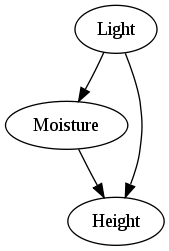
\includegraphics[scale=0.85]{PlantGrowth.png}
    \caption{Bayes Net considered within the plant growth study}
    \label{BNPlant}
  \end{center}
\end{figure}

Both variables $Light$ and $Moisture$ are categorical variables whith the following attributes :  
\begin{itemize}
   \item $Light$ has 2 attributes : $Dim$ which refers to the darkness and $Bright$ which refers to plain light situations,
   \item $Moisture$ has 2 attributes : $Dry$ which refers to dry air situations and $Wet$ which refers to wet air situations.
\end{itemize}
$Height$ is a continuous variable which has to be discretized for the Bayes Net use. \\

The next step is the quantification of the  Bayes Net. According to the data, we propose the following quantification. \\
The variable $Light$ is quantified as follows : 
\begin{itemize}
   \item  $Light="Dim$ with a probability of 0.25,
   \item  $Light=Bright$ with a probability of 0.75.
\end{itemize}

The influence of $Light$ on $Moisture$ is modelized by :
\begin{itemize}
   \item when $Light=Dim$ then  $Moisture=Dry$ with a probability of 0.2 and  $Moisture=Wet$ with a probability of 0.8,
   \item when $Light=Bright$ then  $Moisture=Dry$ with a probability of 0.6 and  $Moisture=Wet$ with a probability of 0.4.
\end{itemize}

The influence of $(Light, Moisture)$ on $Height$ is modelized by :
\begin{itemize}
   \item when $Light=Dim$ and $Moisture=Dry$ then $Height$ follows a $Uniform(min=0, max=20)$ distribution,
   \item when $Light=Dim$ and $Moisture=Wet$ then $Height$ follows a $Triangular(min=15, mod=30, max=50)$ distribution,
   \item when $Light=Bright$ and $Moisture=Dry$ then $Height$ follows a $Triangular(min=0, mod=15, max=30)$ distribution,
   \item when $Light=Bright$ and $Moisture=Wet$ then $Height$ follows a $Normal(\mu=90, \sigma=10)$ distribution.
\end{itemize}


\subsubsection{Some results}

We can study the plant growth variability in different situations like  : 
\begin{itemize}
   \item  I put my plant on my balcony : see Figures \ref{PDFHeight} and \ref{CDFHeight}. In that situation, I set none evidence inside the Bayes Net.
   \item  I put my plant in a  place where it is dark all time (in my cellar?) : see Figures \ref{PDFHeightDim} and \ref{CDFHeightDim}. In that situation, I set one evidence inside the Bayes Net : $Light=Dim$.
   \item  I put my plant in a  place where it is moist all time (in my bathroom?) : see Figures \ref{PDFHeightWet} and \ref{CDFHeightWet}. In that situation, I set one evidence inside the Bayes Net : $Moisture=Wet$.
\end{itemize}




\begin{figure}[H]
  \begin{minipage}{10cm}
    \begin{center}
      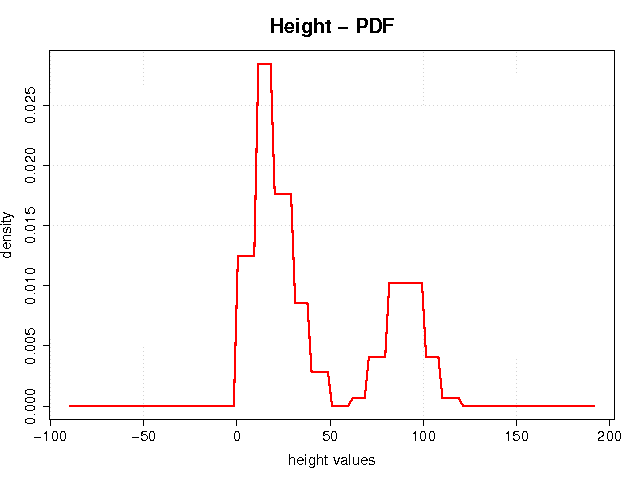
\includegraphics[width=7cm]{Height_PDF.png}
      \caption{Variability of the plant growth on my balcony.}
      \label{PDFHeight}
    \end{center}
  \end{minipage}
  \hfill
  \begin{minipage}{10cm}
    \begin{center}
      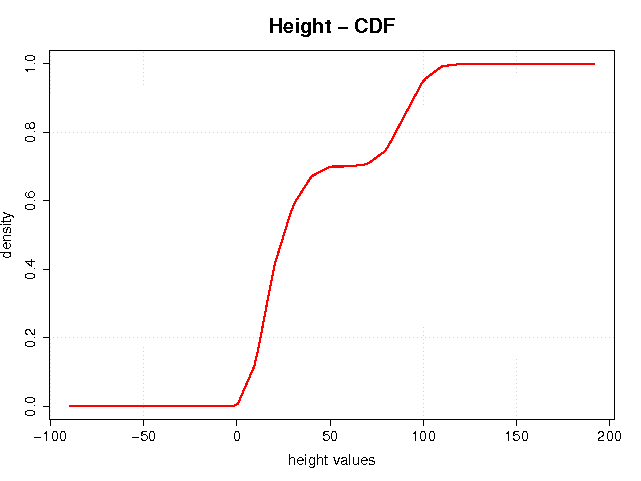
\includegraphics[width=7cm]{Height_CDF.png}
      \caption{Variability of the plant growth on my balcony.}
      \label{CDFHeight}
    \end{center}
  \end{minipage}
\end{figure}



\begin{figure}[H]
  \begin{minipage}{10cm}
    \begin{center}
      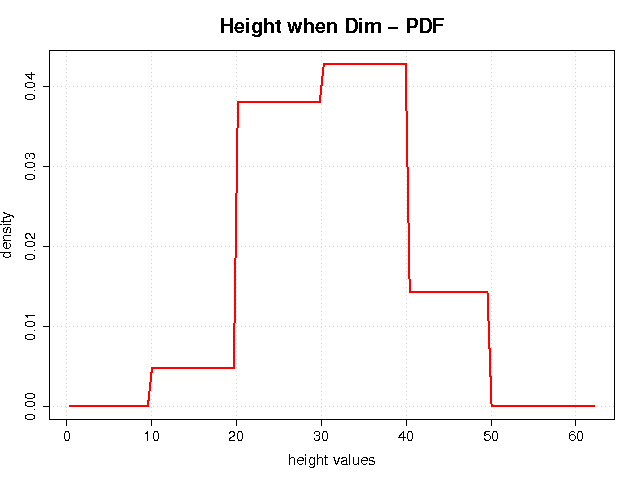
\includegraphics[width=7cm]{Height_PDF_WhenDim.png}
      \caption{Variability of the plant growth in my cellar.}
      \label{PDFHeightDim}
    \end{center}
  \end{minipage}
  \hfill
  \begin{minipage}{10cm}
    \begin{center}
      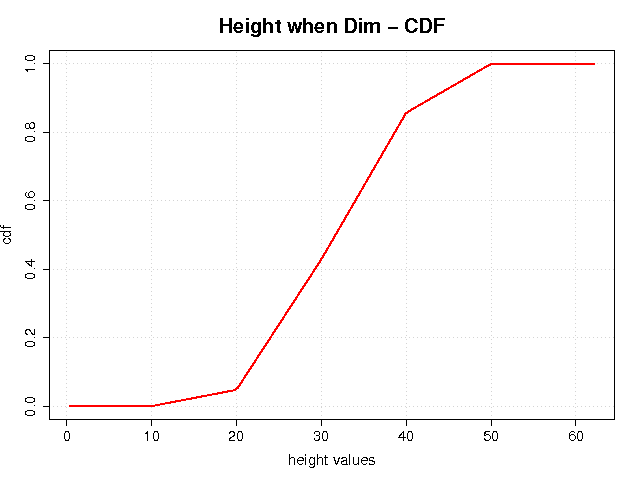
\includegraphics[width=7cm]{Height_CDF_WhenDim.png}
      \caption{Variability of the plant growth in in my cellar.}
      \label{CDFHeightDim}
    \end{center}
  \end{minipage}
\end{figure}


\begin{figure}[H]
  \begin{minipage}{10cm}
    \begin{center}
      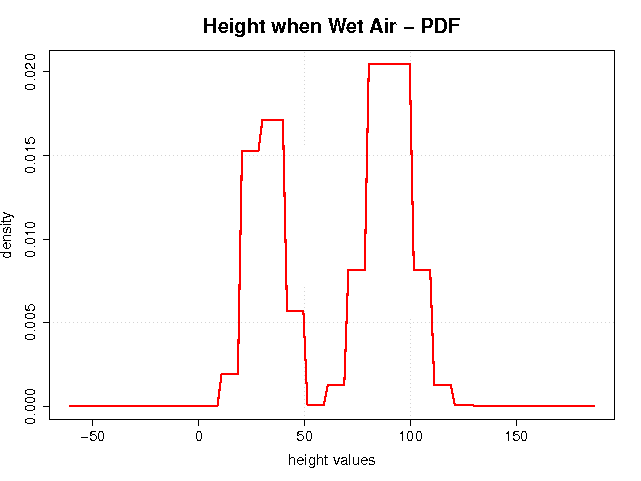
\includegraphics[width=7cm]{Height_PDF_WhenWet.png}
      \caption{Variability of the plant growth in my bathroom.}
      \label{PDFHeightWet}
    \end{center}
  \end{minipage}
  \hfill
  \begin{minipage}{10cm}
    \begin{center}
      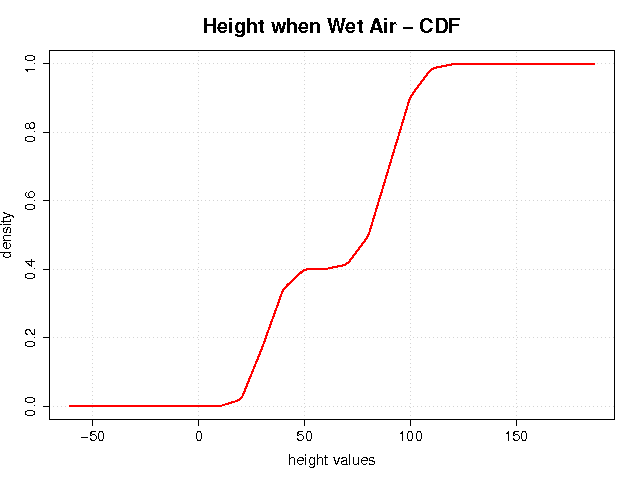
\includegraphics[width=7cm]{Height_CDF_WhenWet.png}
      \caption{Variability of the plant growth in in my bathroom.}
      \label{CDFHeightWet}
    \end{center}
  \end{minipage}
\end{figure}






\subsubsection{Python script}


\begin{lstlisting}
# Load OpenTURNS to manipulate distributions
from openturns import *
# Load pyAgrum to define the Network
from pyAgrum import *
# Load the link between OT and aGrUM
from otagrum import *

# Create an empty BN
netName = "Plant Growth"
myBN = BayesNet(netName)

# Create variables
# LabelizedVar(name, comment, modalities number)
# DiscretizedVar(name, comment)
light = LabelizedVar("Light", "quality of light", 0)
moisture = LabelizedVar("Moisture", "quantity of moisture", 0)
height = DiscretizedVar("Height", "plant growth")

# Create labels and ticks
# light has 2 attributes : Dim and Bright
light.addLabel("Dim")
light.addLabel("Bright")
lightSize = len(light)

# moisture has 2 attributes : Dry and Wet
moisture.addLabel("Dry")
moisture.addLabel("Wet")
moistureSize = len(moisture)


# height has a conditional probability table
# We give here its conditional distributions
# We use some OT distributions
# distribution when Dim and Dry
heightWhenDimAndDry = Uniform(0.0, 20.0)
# distribution when Dim and Wet
heightWhenDimAndWet = Triangular(15.0, 30.0, 50.0)
# distribution when Bright and Dry
heightWhenBrightAndDry = Triangular(0.0, 15.0, 30.0)
# distribution when Bright and Wet
heightWhenBrightAndWet = Normal(90.0, 10.0)

# height is a discretized variable
# We give here its discretized range
data = NumericalPoint(range(0, 180, 10))
# We adapt here its range to its conditional distributions
data = BayesNetAgrum.AdaptGrid(DistributionCollection([
        heightWhenDimAndDry, heightWhenDimAndWet, 
        heightWhenBrightAndDry, heightWhenBrightAndWet
                                                       ]), data)
# We create here the bounds of each local range
#heightSize = data.getSize() - 1
for i in data:
    height.addTick(i)

# Add variables to the net
indexLight    = myBN.add(light)
indexMoisture = myBN.add(moisture)
indexHeight   = myBN.add(height)

# Create arcs
myBN.insertArc(indexLight, indexMoisture)
myBN.insertArc(indexLight, indexHeight)
myBN.insertArc(indexMoisture, indexHeight)

# Create conditional probability tables
# light conditional probability table
myBN.cpt(indexLight)[:]= [0.25, 0.75]

# moisture conditional probability table
# We show the antecedents of moisture with the order in which they were declared
print "moisture Antecedents= ", myBN.cpt(indexMoisture).var_names
myBN.cpt(indexMoisture)[{'Light' : 'Dim'}] = [0.2, 0.8]
myBN.cpt(indexMoisture)[{'Light' : 'Bright'}] = [0.6, 0.4]

# We have to enter some OT distributions 
# whithin aGrUM conditional probability tables
# We show the antecedents of height with the order in which they were declared
print "meight Antecedents= ", myBN.cpt(indexHeight).var_names
# The new class BayesNetAgrum from otagrum is able to marry 
# OT distributions and Agrum conditional probability tables
myBN.cpt(indexHeight)[{'Light': 'Dim', 'Moisture': 'Dry'}]   = 
                BayesNetAgrum.Discretize(heightWhenDimAndDry, data)
myBN.cpt(indexHeight)[{'Light': 'Bright', 'Moisture': 'Dry'}] =
                BayesNetAgrum.Discretize(heightWhenBrightAndDry, data)
myBN.cpt(indexHeight)[{'Light': 'Dim', 'Moisture': 'Wet'}]    = 
                BayesNetAgrum.Discretize(heightWhenDimAndWet, data)
myBN.cpt(indexHeight)[{'Light': 'Bright', 'Moisture': 'Wet'}] = 
                BayesNetAgrum.Discretize(heightWhenBrightAndWet, data)

# Create a BayesNetAgrum object
otbn = BayesNetAgrum(myBN)

# We want to visualize the bayesian network 
# Export to BIF file
otbn.exportToBIFFile(netName+".bif")
# Visualize the graph
otbn.draw(netName)


# Get the distribution of the variable "Height"
heightDistribution = otbn.getMarginal("Height")

# You are whithin Open TURNS : use the distribution the way you want
# Print its caracteristics
print "heightDistribution =", heightDistribution
# Draw its PDf and CDF
heightDistributionPDF = heightDistribution.drawPDF()
heightDistributionPDF.setTitle("Height - PDF")
heightDistributionPDF.setXTitle("height values")
heightDistributionPDF.setYTitle("density")
heightDistributionPDF_draw = heightDistributionPDF.getDrawable(0)
heightDistributionPDF_draw.setLegendName("")
heightDistributionPDF.setDrawable(heightDistributionPDF_draw,0)
heightDistributionPDF.draw("Height_PDF")
heightDistributionCDF = heightDistribution.drawCDF()
heightDistributionCDF.setTitle("Height - CDF")
heightDistributionCDF.setXTitle("height values")
heightDistributionCDF.setYTitle("density")
heightDistributionCDF_draw = heightDistributionCDF.getDrawable(0)
heightDistributionCDF_draw.setLegendName("")
heightDistributionCDF.setDrawable(heightDistributionCDF_draw,0)
heightDistributionCDF.draw("Height_CDF")


# Perform inference

##############################################################
# Example 1 : it is sunny : "Light" == "Bright"

# First, set evidence
otbn.setEvidence("Light", "Bright")

# Get the distribution of the variable "Height"
heightDistribution_Bright = otbn.getMarginal("Height")

# You are whithin Open TURNS : use the distribution the way you want
# Print its caracteristics
print "Height Distribution when Bright =", heightDistribution_Bright
print "Probability (height > 40cm) = ", 1-heightDistribution_Bright.computeCDF(40)
print ""
# Draw its PDF and CDF
heightDistributionPDF_Bright = heightDistribution_Bright.drawPDF()
heightDistributionPDF_Bright.setTitle("Height when Bright - PDF")
heightDistributionPDF_Bright.setXTitle("height values")
heightDistributionPDF_Bright.setYTitle("density")
heightDistributionPDF_Bright_draw = heightDistributionPDF_Bright.getDrawable(0)
heightDistributionPDF_Bright_draw.setLegendName("")
heightDistributionPDF_Bright.setDrawable(heightDistributionPDF_Bright_draw,0)
heightDistributionPDF_Bright.draw("Height_PDF_WhenBright")

heightDistributionCDF_Bright = heightDistribution_Bright.drawCDF()
heightDistributionCDF_Bright.setTitle("Height when Bright - CDF")
heightDistributionCDF_Bright.setXTitle("height values")
heightDistributionCDF_Bright.setYTitle("cdf")
heightDistributionCDF_Bright_draw = heightDistributionCDF_Bright.getDrawable(0)
heightDistributionCDF_Bright_draw.setLegendName("")
heightDistributionCDF_Bright.setDrawable(heightDistributionCDF_Bright_draw,0)
heightDistributionCDF_Bright.draw("Height_CDF_WhenBright")

##############################################################
# Example 2 : the atmosphere is very wet : "Moisture" == "Wet"

# First, erase previous evidences!
otbn.eraseEvidences()
# Set evidence
otbn.setEvidence("Moisture", "Wet")

# Get the distribution of the variable "Light"
lightDistribution_Wet = otbn.getMarginal("Light")
print "Light distribution when Wet Air = "
print "Proba(Dim) = ", lightDistribution_Wet.getParametersCollection()[0][0]
print "Proba(Bright) = ", lightDistribution_Wet.getParametersCollection()[0][1]
print ""

# Get the distribution of the variable "Height"
heightDistribution_Wet = otbn.getMarginal("Height")

# You are whithin Open TURNS : use the distribution the way you want
# Print its caracteristics
print "Height Distribution when Wet Air =", heightDistribution_Wet
print "Probability (height > 40cm) = ", 1-heightDistribution_Wet.computeCDF(40)
print ""
# Draw its PDF and CDF
heightDistributionPDF_Wet = heightDistribution_Wet.drawPDF()
heightDistributionPDF_Wet.setTitle("Height when Wet Air - PDF")
heightDistributionPDF_Wet.setXTitle("height values")
heightDistributionPDF_Wet.setYTitle("density")
heightDistributionPDF_Wet_draw = heightDistributionPDF_Wet.getDrawable(0)
heightDistributionPDF_Wet_draw.setLegendName("")
heightDistributionPDF_Wet.setDrawable(heightDistributionPDF_Wet_draw,0)
heightDistributionPDF_Wet.draw("Height_PDF_WhenWet")
heightDistributionCDF_Wet = heightDistribution_Wet.drawCDF()
heightDistributionCDF_Wet.setTitle("Height when Wet Air - CDF")
heightDistributionCDF_Wet.setXTitle("height values")
heightDistributionCDF_Wet.setYTitle("density")
heightDistributionCDF_Wet_draw = heightDistributionCDF_Wet.getDrawable(0)
heightDistributionCDF_Wet_draw.setLegendName("")
heightDistributionCDF_Wet.setDrawable(heightDistributionCDF_Wet_draw,0)
heightDistributionCDF_Wet.draw("Height_CDF_WhenWet")


##############################################################
# Example 3 : there is no light : "Light" == "Dim"

# First, add one more  evidence
otbn.setEvidence("Light", "Dim")

# Get the distribution of the variable "Height"
heightDistribution_Dim = otbn.getMarginal("Height")

# You are whithin Open TURNS : use the distribution the way you want
# Print its caracteristics
print "Height Distribution when Dim =", heightDistribution_Dim
print "Probability (height > 40cm) = ", 1-heightDistribution_Dim.computeCDF(40)
print ""
# Draw its PDf and CDF
heightDistributionPDF_Dim = heightDistribution_Dim.drawPDF()
heightDistributionPDF_Dim.setTitle("Height when Dim - PDF")
heightDistributionPDF_Dim.setXTitle("height values")
heightDistributionPDF_Dim.setYTitle("density")
heightDistributionPDF_Dim_draw = heightDistributionPDF_Dim.getDrawable(0)
heightDistributionPDF_Dim_draw.setLegendName("")
heightDistributionPDF_Dim.setDrawable(heightDistributionPDF_Dim_draw,0)
heightDistributionPDF_Dim.draw("Height_PDF_WhenDim")

heightDistributionCDF_Dim = heightDistribution_Dim.drawCDF()
heightDistributionCDF_Dim.setTitle("Height when Dim - CDF")
heightDistributionCDF_Dim.setXTitle("height values")
heightDistributionCDF_Dim.setYTitle("cdf")
heightDistributionCDF_Dim_draw = heightDistributionCDF_Dim.getDrawable(0)
heightDistributionCDF_Dim_draw.setLegendName("")
heightDistributionCDF_Dim.setDrawable(heightDistributionCDF_Dim_draw,0)
heightDistributionCDF_Dim.draw("Height_CDF_WhenDim")
\end{lstlisting}









%%%%%%%%%%%%%%%%%%%%%%%%%%%%%%%%%%%%%%%%%%%%%
\newpage \subsection{Your study}

It's up to you to propose one new very interesting example! ...